\subsection{モデル概要}
入力された動画を[優美なダンス,普通のダンス,その他の動作]に分類するネットワークを作成した.
ネットワーク内での分類手順として
\begin{enumerate}
  \item 動画を下記で説明する二値化手法で編集する.
  \item 二値データと,それに対応するピクセル番号を畳み込む.
  \item 二つのデータを足し合わせる.
  \item Transformer Encoderに通した後,全結合し,Softmaxにかける.
\end{enumerate}
のような順序で計算した.
最適化アルゴリズムにAdam\cite{adam},損失関数に交差エントロピー誤差(\ref{entropy})を使用した.
\begin{equation}
  H(p, q) = -\sum_{i}p_i\log q_i
  \label{entropy}
\end{equation}
プログラミング言語にPython,モジュールは主にPytorch,Numpy,Cv2,Pickleを用いた.

\begin{figure}[b]
  \begin{center}
    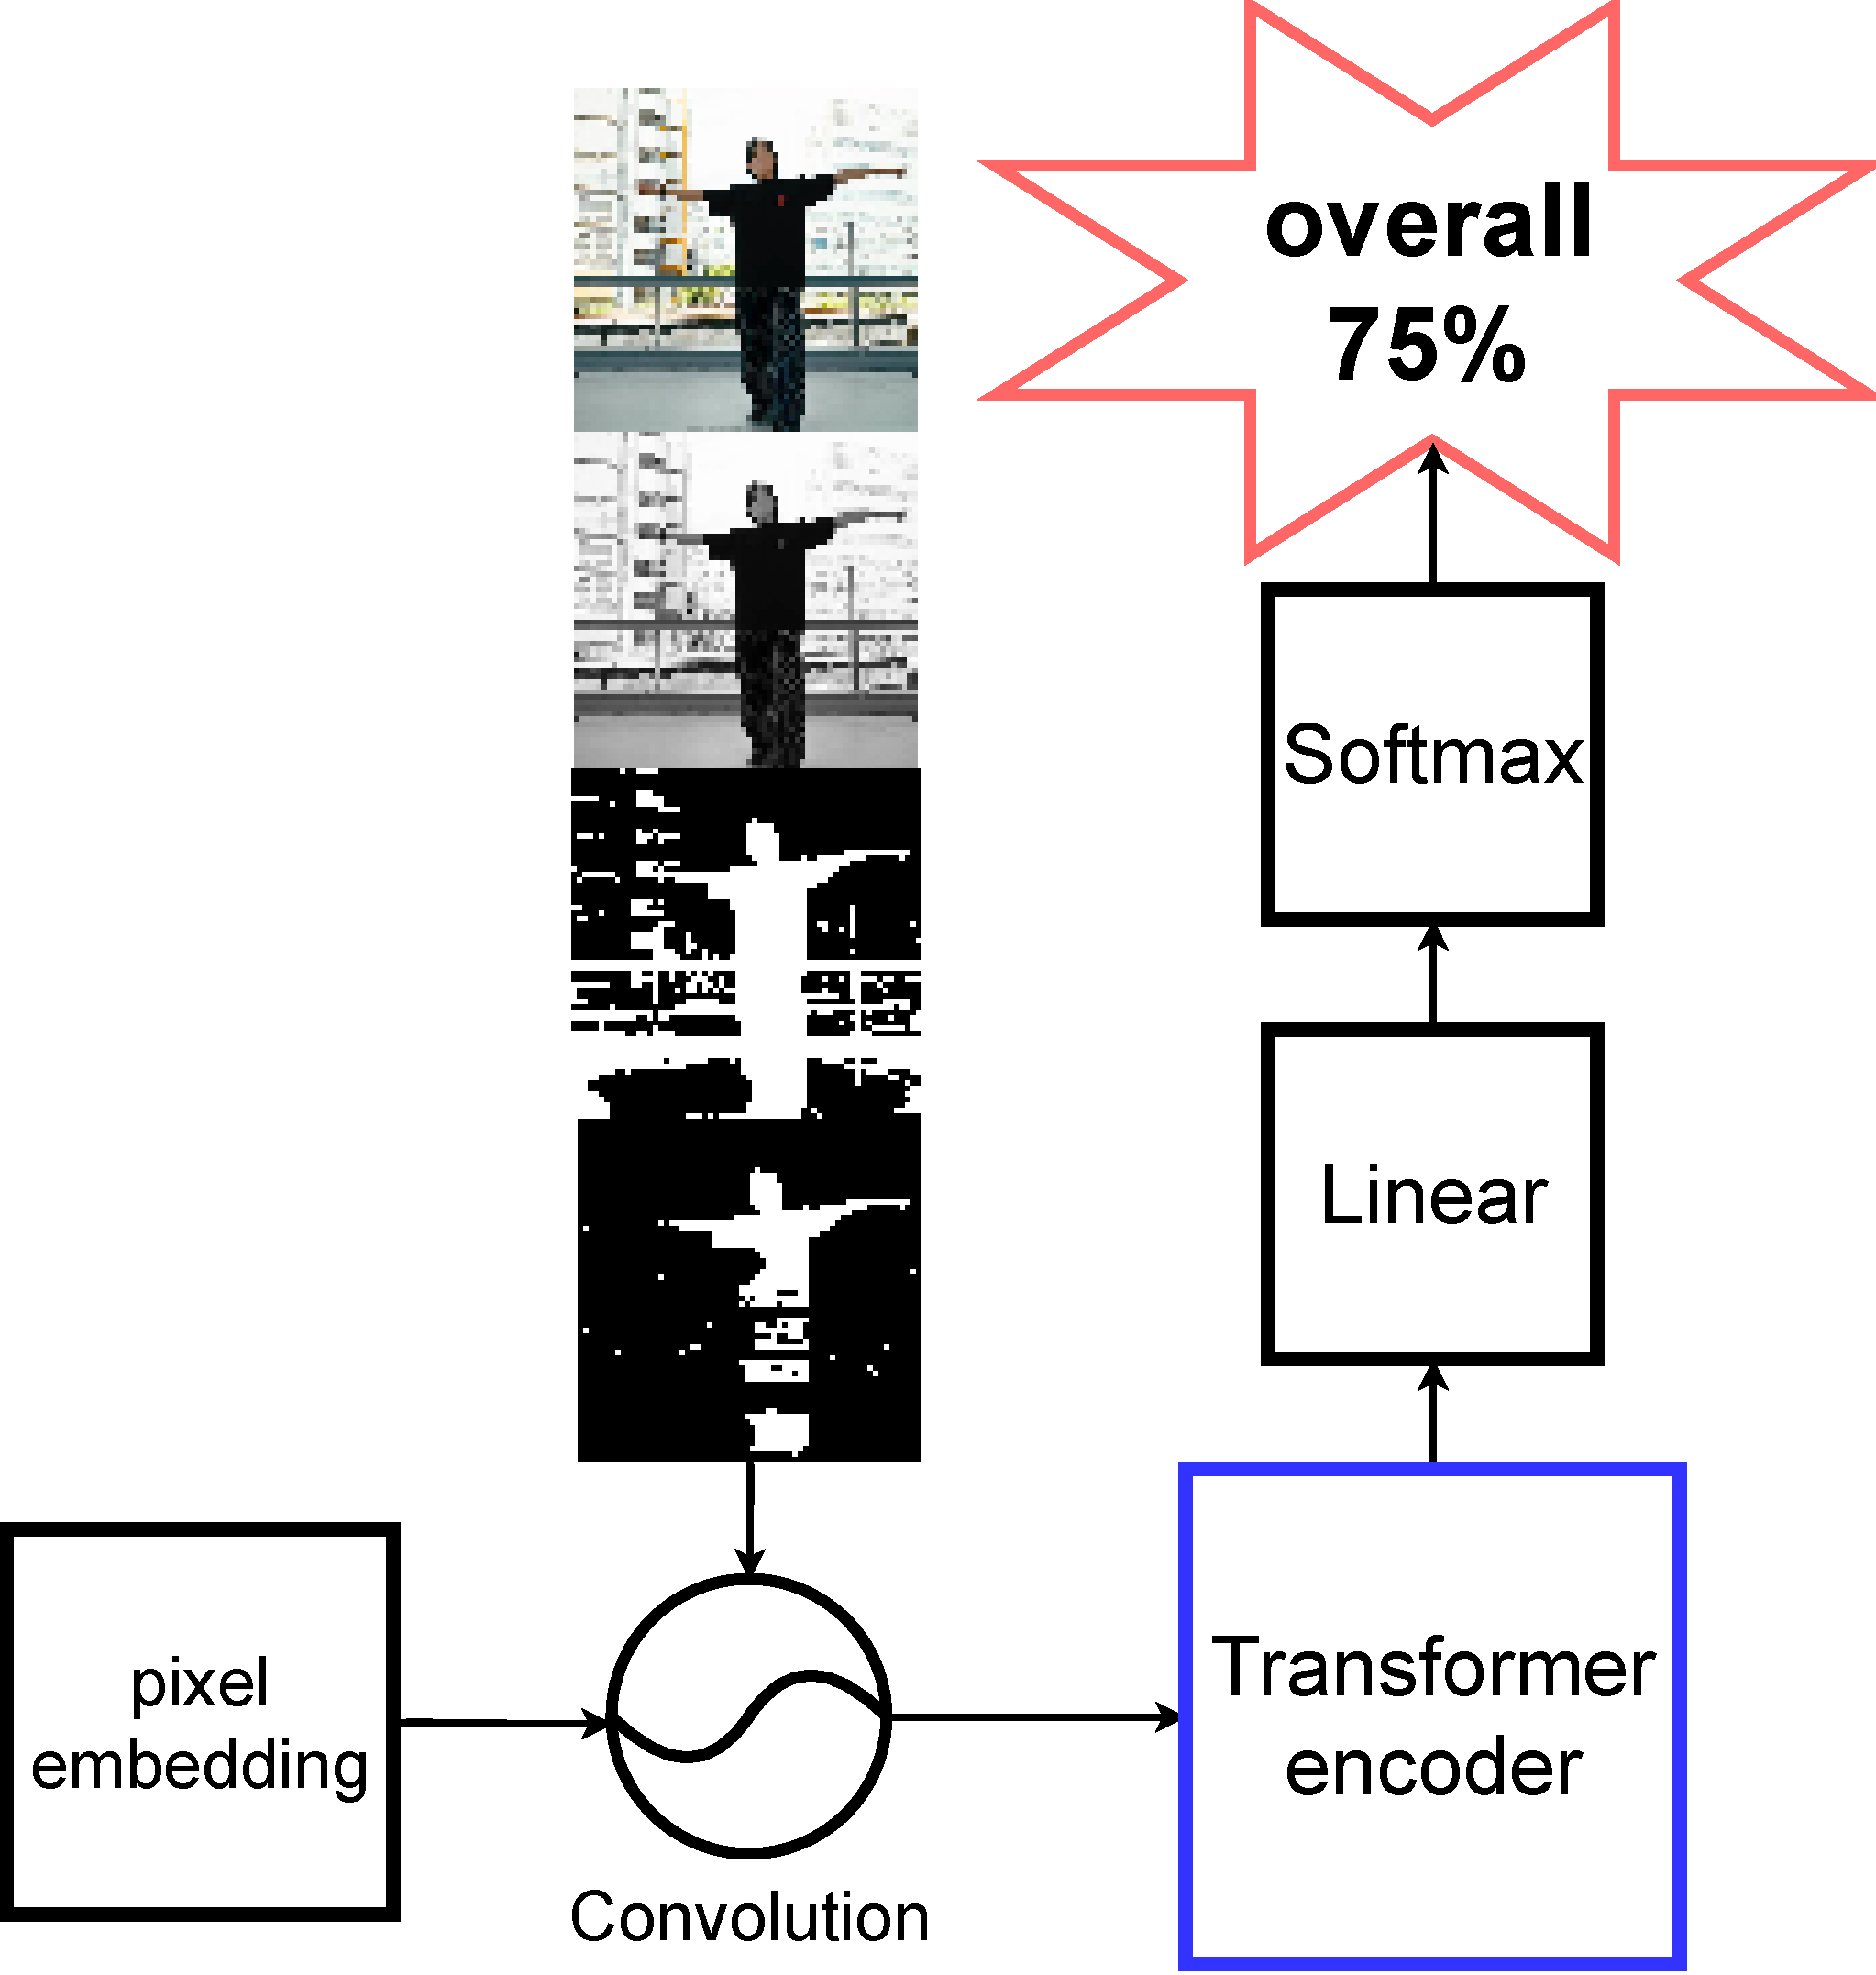
\includegraphics[width=80mm]{images/easy_chart.pdf}
  \end{center}
  \caption{モデル概要}
  \label{easy_chart}
\end{figure}

\clearpage

\subsection{使用する動画データ}
動画は\ref{video_data}を使用した.
\begin{table}[t]
  \begin{center}
    \begin{tabular}{|c|c|c|} \hline
      \ & 学習用 & 推論用 \\ \hline
      優美なダンス
        & \cite{jpn}\cite{china}\cite{ballet}\cite{thai}\cite{jpn2}
        & \cite{balletgroup}\cite{jpngroup}\cite{chinagroup}\cite{belly}
      \\ \hline
      普通のダンス
        & \cite{ariana}\cite{kadokawa}\cite{bts}\cite{manolo}\cite{aito}
        & \cite{btsgroup}\cite{arashi}\cite{hyoga}\cite{legit}
      \\ \hline
      その他の動作
        & \cite{radio}\cite{posing}\cite{boxing}\cite{running}\cite{shinkokyu}\cite{leaves}
        & \cite{radio2}
      \\ \hline
    \end{tabular}
  \end{center}
  \caption{使用した動画データ}
  \label{video_data}
\end{table}

\subsection{ネットワーク構造}

\subsection{精度}